\section{Methodology and Implementation}
\label{sec:solution}

We implement the sequential algorithm described by Şen and Diner \cite{Sen2024Futoshiki} and apply the parallel programming methodologies covered in this course. Our approach follows a systematic progression: first implementing their list coloring-based sequential solver, then developing MPI, OpenMP, and hybrid parallelizations using the techniques studied.

The implementation translates their theoretical constraint propagation approach into working code, then explores how different parallelization paradigms can be applied to the resulting backtracking search problem.

\subsection{Sequential Algorithm Implementation}
\label{subsec:paper_implementation}
We begin by implementing the sequential algorithm described in the chosen paper. Their approach transforms Futoshiki into a list coloring problem, enabling constraint propagation to reduce the search space before applying backtracking.

\subsection{Sequential Algorithm Implementation}
\label{subsec:paper_implementation}
We implement the list coloring transformation detailed by Şen and Diner \cite{Sen2024Futoshiki}. Translating their theoretical approach into working code required several key implementation decisions that significantly impact the subsequent parallelization strategies.

\subsubsection{Pre-coloring: Search Space Reduction}
\label{subsubsec:precoloring}
The pre-coloring phase, implemented in \texttt{compute\_pc\_lists}, computes a "possible color list" (pc\_list) for each cell through iterative constraint propagation:

\begin{enumerate}
    \item \textbf{Initialization:} Empty cells receive pc\_lists containing all values 1 to N. Pre-filled cells contain only their given value.
    
    \item \textbf{Inequality Filtering:} The \texttt{filter\_possible\_colors} function removes values that violate inequality constraints. For instance, if cell A $>$ cell B and A's pc\_list = \{1, 2\}, then B cannot contain values $<$ 2.
    
    \item \textbf{Uniqueness Propagation:} When a cell's pc\_list reduces to a single value, \texttt{process\_uniqueness} removes that value from all other cells in the same row and column. To continue with our example, as B can have value 1 and 2, and as A can have $n < 2$, it would mean that A is going to hold 1 as it is the only integer strictly lower than 2, and B therefore would hold 2, as its pc\_list had two values and we need to respect the \textit{Latin Square} property.
    
    \item \textbf{Iteration:} The previous two steps repeat until no further reductions occur, ensuring maximal constraint propagation.
\end{enumerate}

This implementation typically achieves the 70-90\% search space reduction reported in the paper, creating the foundation for effective parallelization.

\subsubsection{Backtracking Implementation}
\label{subsubsec:backtrack_with_csp}
The core solving algorithm translates the paper's constrained search into the recursive function \texttt{seq\_color\_g}:

\begin{lstlisting}[language=C, caption=Sequential backtracking implementation, label={listing:seq_implementation}]
bool seq_color_g(Futoshiki* puzzle, 
                 int solution[MAX_N][MAX_N], 
                 int row, int col) {
    if (row >= puzzle->size) return true;
    if (col >= puzzle->size) 
        return seq_color_g(puzzle, solution, 
                          row + 1, 0);
    
    if (puzzle->board[row][col] != EMPTY) {
        solution[row][col] = 
            puzzle->board[row][col];
        return seq_color_g(puzzle, solution, 
                          row, col + 1);
    }
    
    for (int i = 0; 
         i < puzzle->pc_lengths[row][col]; i++) {
        int color = puzzle->pc_list[row][col][i];
        if (safe(puzzle, row, col, 
                 solution, color)) {
            solution[row][col] = color;
            if (seq_color_g(puzzle, solution, 
                            row, col + 1))
                return true;
            solution[row][col] = EMPTY;
        }
    }
    return false;
}
\end{lstlisting}

The implementation explores only values in each cell's reduced \texttt{pc\_list}, with the \texttt{safe} function validating constraint compliance. This creates the sequential baseline that serves as both the performance benchmark and the building block for parallel implementations.

\textbf{Correctness Foundation for Parallelization:} A critical property of Futoshiki puzzles is that each valid instance has exactly one unique solution. This characteristic enables safe parallel implementation with early termination—when any worker discovers the solution, all other workers can immediately halt without risking loss of correctness.

\subsection{Parallelization Strategy}
\label{subsec:parallel_implementation}
The sequential implementation reveals parallelization opportunities in the backtracking phase. Since constraint propagation completes quickly in polynomial time, we focus on parallelizing the exponential backtracking search, following Amdahl's Law \cite{ahmdals_law} principles by targeting the computationally dominant phase.

All three parallel implementations share a common challenge: how to distribute the irregular search tree effectively across available workers. We address this through a dynamic work generation framework that creates appropriate work units based on available parallelism.

\subsubsection{Dynamic Work Generation Framework}
\label{subsubsec:dynamic_load_balancing}
A key implementation challenge was developing a work distribution strategy suitable for all three parallelization paradigms. Rather than static partitioning, we implemented an adaptive approach in \texttt{parallel.c} that analyzes the search tree to generate appropriate work units.

\begin{lstlisting}[language=C, caption=Dynamic depth calculation for work generation, label={listing:work_generation}]
int calculate_distribution_depth(
    Futoshiki* puzzle, int num_workers) {
    int empty_cells[MAX_N * MAX_N][2];
    int num_empty = find_empty_cells(
        puzzle, empty_cells);
    
    for (int d = 1; d <= num_empty; d++) {
        long long job_count = 
            count_valid_assignments_recursive(
                puzzle, solution, empty_cells, 
                num_empty, 0, d);
        
        if (job_count > num_workers) {
            log_info("Depth %d generates %lld units", 
                     d, job_count);
            return d;
        }
    }
    return num_empty;
}
\end{lstlisting}

The algorithm explores progressively deeper levels of the search tree until generating sufficient work units. Each work unit represents a partial solution path, ensuring that workers receive meaningful chunks of computation while maintaining load balance. This approach addresses the irregular nature of Futoshiki's constraint patterns that make static distribution ineffective.

\subsubsection{MPI Implementation: Master-Worker Pattern}
\label{subsubsec:mpi_implementation}
Following the distributed-memory programming techniques from the course, we implemented a master-worker paradigm suitable for cluster environments. The design applies the message-passing concepts studied:
\begin{enumerate}
\textbf{Master Process (Rank 0):}
\begin{itemize}
    \item Performs precoloring and fills out a basic version of the puzzle
    \item Based on the configuration factor given, decides the ratio of jobs to CPUs by evaluating the depth of the backtracking approach and opens the port to listen to the workers
    \item Sends 1 job to each worker via the \texttt{TAG\_WORK\_ASSIGNMENT}
    \item If a worker does not solve the job, it receives the message and sends a new job via the same tag. If the solution is found, it broadcasts to every other worker to stop via \texttt{TAG\_TERMINATE}. This leverages the unique solution property of Futoshiki puzzles for correctness
    \item Collects the solution found and sends it to the user
\end{itemize}

\textbf{Worker Processes (Ranks 1 to P-1):}
\begin{itemize}
    \item Poll master by asking for a job to solve via \texttt{TAG\_WORK\_REQUEST}
    \item Try to solve the precolored puzzle given. If successful, send \texttt{TAG\_SOLUTION\_FOUND} followed by \texttt{TAG\_SOLUTION\_DATA}, otherwise send another \texttt{TAG\_WORK\_REQUEST}
    \item Upon receiving \texttt{TAG\_TERMINATE} from the master, gracefully shut down as this indicates a solution was found
\end{itemize}

\begin{figure}[htbp]
\centering
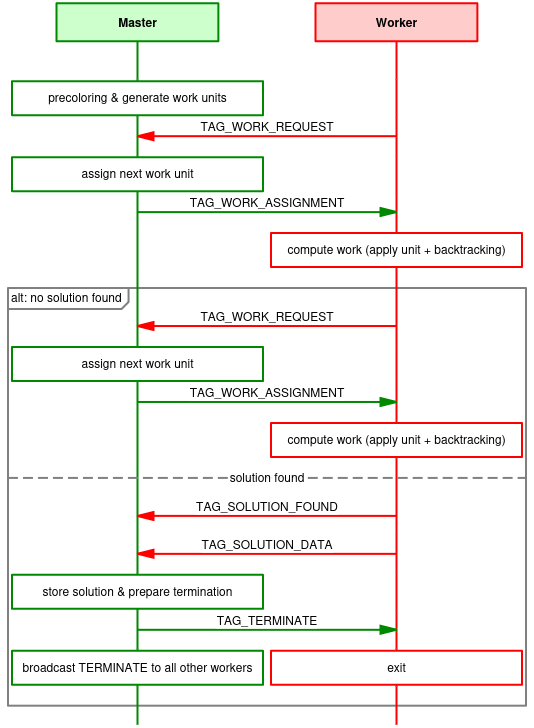
\includegraphics[width=0.9\linewidth]{imgs/mpi_msc.png}
\caption{MPI Master-Worker communication sequence showing the request-assign-solve-report-terminate protocol}
\label{fig:mpi_sequence}
\end{figure}

The communication protocol uses five message tags to coordinate the distributed solving process:

\begin{lstlisting}[language=C, caption=MPI communication protocol, label={listing:mpi_tags}]
typedef enum {
    TAG_WORK_REQUEST = 1,
    TAG_SOLUTION_FOUND = 2,
    TAG_SOLUTION_DATA = 3,
    TAG_TERMINATE = 4,
    TAG_WORK_ASSIGNMENT = 5
} MessageTag;
\end{lstlisting}

\textbf{Implementation Note:} When only one MPI process is available, the implementation automatically falls back to the sequential algorithm as only a master and no worker would be available.

This design enables dynamic load balancing as workers request work only when ready, automatically handling heterogeneous performance and variable work unit difficulty typical in constraint satisfaction problems.


\subsubsection{OpenMP Implementation: Task-Based Parallelism}
\label{subsubsec:omp_implementation}
Following the shared-memory programming techniques from the course, we implemented task-based parallelism using OpenMP. After generating work units, the master thread spawns OpenMP tasks that are dynamically scheduled across available threads.

From a high-level perspective, once the precoloring phase is performed, the master thread gives each worker a puzzle with a partial solution. When any worker finds the complete solution, it sets the \texttt{found\_solution} flag to true, effectively stopping other threads from continuing unnecessary work.

\begin{lstlisting}[language=C, caption=OpenMP task-based implementation, label={listing:omp_implementation}]
#pragma omp parallel
{
    #pragma omp single
    {
        for (int i = num_work_units - 1; 
             i >= 0 && !found_solution; i--) {
            #pragma omp task firstprivate(i) \
                        shared(found_solution)
            {
                if (!found_solution) {
                    int local_solution[MAX_N][MAX_N];
                    apply_work_unit(puzzle, 
                        &work_units[i], local_solution);
                    
                    if (seq_color_g(puzzle, 
                        local_solution, 
                        start_row, start_col)) {
                        #pragma omp critical
                        {
                            if (!found_solution) {
                                found_solution = true;
                                memcpy(solution, 
                                    local_solution, 
                                    sizeof(local_solution));
                            }
                        }
                    }
                }
            }
        }
        #pragma omp taskwait
    }
}
\end{lstlisting}

\textbf{Key Implementation Features:}
\begin{itemize}
    \item \textbf{Dynamic Scheduling:} OpenMP runtime automatically balances tasks across threads, adapting to varying work unit difficulty without explicit load balancing code.
    \item \textbf{Early Termination:} The shared \texttt{found\_solution} variable enables early termination across all threads. This provides substantial speedup since probabilistically, the solution is unlikely to be found in the very last work unit processed.
    \item \textbf{Configurable Task Factor:} The dynamic task generation factor allows tuning the ratio between available threads and generated jobs, enabling control over the computational "stress" applied to the system.
\end{itemize}

\textbf{Single-Thread Fallback Design Decision:}
An implementation detail worth noting is our fallback to the sequential algorithm when only one thread is available. While OpenMP can run with a single thread, we chose this approach for two reasons:
\begin{itemize}
    \item \textbf{Overhead Avoidance:} Single-threaded OpenMP incurs code expansion and metadata overhead during compilation that provides no benefit when parallelism isn't utilized.
    \item \textbf{Interface Consistency:} To enable meaningful performance comparisons with MPI, we maintain similar design patterns across implementations.
\end{itemize}

\textbf{Shared Memory vs. Message Passing:}
Unlike the MPI implementation, this approach leverages shared memory rather than message passing. Variables are explicitly declared as shared or private using OpenMP clauses, and early termination occurs through the shared variable mechanism rather than broadcast messages.

\textbf{Data Dependency Analysis}

Data dependency analysis in parallel programming identifies relationships between different parts of code that affect execution order. This analysis ensures parallel tasks operate without conflicts, preventing race conditions and maintaining correctness while enabling efficient parallelization.

The analysis focuses on the core parallel loop where tasks process work units concurrently. Table \ref{tab:omp_dependencies_detailed} presents the complete dependency analysis for the critical shared variables.

\begin{table}[htbp]
\caption{Detailed Data Dependencies in OpenMP Task Implementation}
\begin{center}
\small
\begin{tabular}{@{}lcccccc@{}}
\toprule
\textbf{Memory} & \multicolumn{2}{c}{\textbf{Earlier Statement}} & \multicolumn{2}{c}{\textbf{Later Statement}} & \textbf{Loop} & \textbf{Dependency} \\
\textbf{Location} & \textbf{Line} & \textbf{Access} & \textbf{Line} & \textbf{Access} & \textbf{Carried?} & \textbf{Type} \\
\midrule
found\_solution & 43 & read & 44 & write & ✗ & anti \\
found\_solution & 44 & write & 29 & read & ✓ & flow \\
found\_solution & 44 & write & 32 & read & ✓ & flow \\
found\_solution & 44 & write & 43 & read & ✓ & flow \\
found\_solution & 44 & write & 44 & write & ✓ & output \\
solution & 45 & write & 45 & write & ✓ & output \\
\bottomrule
\end{tabular}
\end{center}
\label{tab:omp_dependencies_detailed}
\end{table}

\textbf{Dependency Analysis Results:}

\begin{enumerate}
    \item \textbf{Anti-dependency (Line 43→44, same task):} Within each task, the read of \texttt{found\_solution} at line 43 followed by potential write at line 44 creates an anti-dependency. This is benign since it occurs sequentially within the same thread.
    
    \item \textbf{Flow dependencies (Lines 44→29, 44→32, 44→43):} When one task writes \texttt{found\_solution = true}, other tasks must see this update to terminate early. Without proper synchronization, tasks might continue processing after a solution is found, causing inefficiency but not incorrectness.
    
    \item \textbf{Output dependencies (Lines 44→44, 45→45):} Multiple tasks finding solutions simultaneously could write to the same memory locations concurrently, causing undefined behavior. This is not possible by the definition of a Futoshiki puzzle.
\end{enumerate}

\textbf{Mitigation Strategies Applied:}

The implementation employs several OpenMP synchronization mechanisms to address these dependencies:

\begin{itemize}
    \item \texttt{firstprivate(i)}: Ensures each task has its own copy of the loop variable, preventing interference between tasks
    \item \texttt{shared(found\_solution)}: Explicitly declares shared access to the termination flag for memory coherence
    \item \texttt{\#pragma omp critical}: Provides mutual exclusion for the check-then-act pattern, ensuring only one task can update shared state atomically
    \item \texttt{\#pragma omp taskwait}: Prevents premature resource deallocation while tasks are still executing
\end{itemize}

The critical section implements a double-check pattern: tasks first check \texttt{found\_solution} outside the critical section for efficiency, then check again inside for correctness. This minimizes time spent in the critical section while ensuring race-free updates to both the solution flag and the solution array.

\subsubsection{Hybrid Implementation: Combining MPI and OpenMP}
\label{subsubsec:hybrid_implementation}

The hybrid approach represents the culmination of applying multiple methodologies to a single problem. Following the principles of hierarchical parallelization, we combine MPI's distributed-memory capabilities with OpenMP's shared-memory efficiency in a two-layer architecture.

\textbf{Two-Layer Design Philosophy:}
Our hybrid implementation follows a systematic layering approach to maximize the benefits of both paradigms:

\begin{itemize}
    \item \textbf{Outer Layer (Inter-node):} MPI distributes coarse-grained work units across cluster nodes, handling the master-worker coordination and work distribution logic identical to the pure MPI implementation.
    \item \textbf{Inner Layer (Intra-node):} OpenMP parallelizes the solving of each work unit within individual nodes, applying the task-based approach from our OpenMP implementation.
\end{itemize}

This design abstracts the two approaches while maintaining common APIs across implementations, enabling direct performance comparisons and modular development.

\textbf{Implementation Strategy:}
The hybrid approach reuses the established MPI communication protocol while substituting the sequential solving step with our OpenMP solver. This demonstrates how the methodologies can be composed hierarchically:

\begin{lstlisting}[language=C, caption=Hybrid worker combining MPI and OpenMP, label={listing:hybrid_worker}]
static void hybrid_worker(Futoshiki* puzzle) {
    WorkUnit work_unit;
    MPI_Status status;
    
    while (true) {
        // MPI layer: request work from master
        int request = 1;
        MPI_Send(&request, 1, MPI_INT, 0, 
                 TAG_WORK_REQUEST, MPI_COMM_WORLD);
        MPI_Recv(&work_unit, sizeof(WorkUnit), 
                 MPI_BYTE, 0, MPI_ANY_TAG, 
                 MPI_COMM_WORLD, &status);
        
        if (status.MPI_TAG == TAG_TERMINATE) break;
        
        // Apply work unit to create sub-puzzle
        Futoshiki sub_puzzle;
        memcpy(&sub_puzzle, puzzle, sizeof(Futoshiki));
        apply_work_unit(&sub_puzzle, &work_unit, 
                       sub_puzzle.board);
        
        // OpenMP layer: solve using task-based parallelism
        int local_solution[MAX_N][MAX_N];
        if (omp_solve(&sub_puzzle, local_solution)) {
            // MPI layer: report solution back to master
            int found_flag = 1;
            MPI_Send(&found_flag, 1, MPI_INT, 0, 
                    TAG_SOLUTION_FOUND, MPI_COMM_WORLD);
            MPI_Send(local_solution, MAX_N * MAX_N, 
                    MPI_INT, 0, TAG_SOLUTION_DATA, 
                    MPI_COMM_WORLD);
            break;
        }
    }
}
\end{lstlisting}

\textbf{Design Benefits and Trade-offs:}
The hybrid approach demonstrates several key principles from parallel computing:

\begin{enumerate}
    \item \textbf{Hierarchical Decomposition:} Work is decomposed at two levels—coarse-grained distribution via MPI and fine-grained task parallelism via OpenMP, matching the hardware hierarchy of clusters with multi-core nodes.
    
    \item \textbf{Communication Minimization:} By using OpenMP within nodes, we reduce the number of MPI processes needed, decreasing inter-node communication overhead which is typically orders of magnitude more expensive than intra-node synchronization.
    
    \item \textbf{Resource Utilization:} The approach can better exploit modern cluster architectures where each node contains multiple cores, using MPI for scalability across nodes and OpenMP for efficiency within nodes.
    
    \item \textbf{Implementation Modularity:} By maintaining common interfaces, the hybrid approach leverages existing MPI and OpenMP implementations without requiring complete redesign.
\end{enumerate}

\textbf{Configuration Flexibility:}
The hybrid model supports various process-thread combinations, enabling exploration of different resource allocation strategies. For a fixed number of computational units, one can configure:
\begin{itemize}
    \item \textbf{MPI-heavy:} More processes, fewer threads per process (e.g., 8 processes × 2 threads)
    \item \textbf{OpenMP-heavy:} Fewer processes, more threads per process (e.g., 2 processes × 8 threads)  
    \item \textbf{Balanced:} Equal distribution (e.g., 4 processes × 4 threads)
\end{itemize}

This configurability allows performance tuning based on problem characteristics and hardware topology, demonstrating practical application of parallel programming trade-offs discussed in course materials.

The hybrid implementation showcases how multiple parallelization paradigms can be systematically combined, providing a comprehensive application of methodologies to constraint satisfaction problems.
